\suppnote{Supplementary Note S21. Supporting source-likelihood comparison}
\begin{figure}[H]
\centering
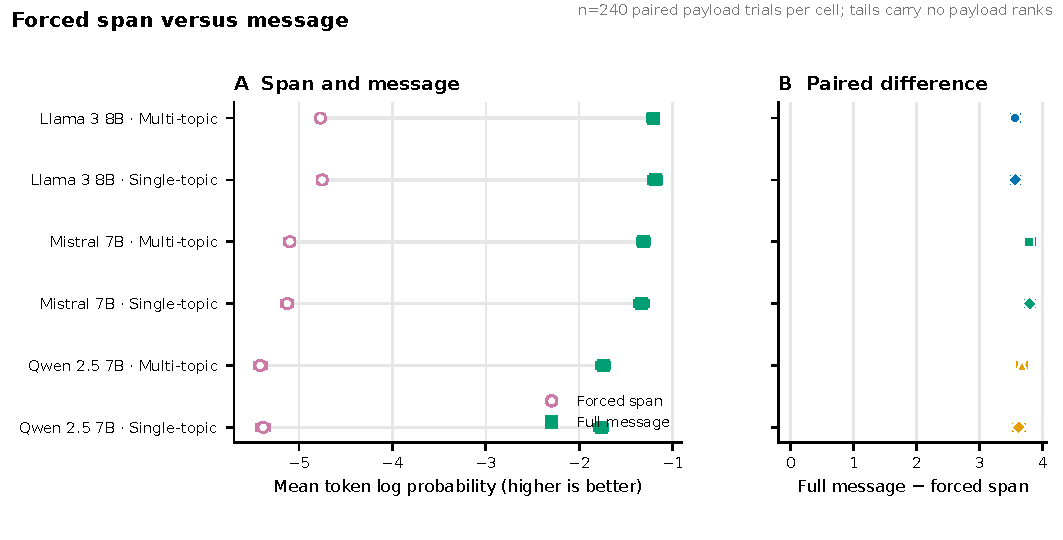
\includegraphics[width=\textwidth]{figures/forced_span_full_message_quality.pdf}
\caption{\label{fig:forced-full}\textbf{Forced span versus full message.} Mean token log probability is paired within 1,440 segmented trials across three models and single-topic or multi-topic schedules, with 240 trials per model schedule cell. Error bars are 2,000 resample paired payload bootstrap 95\% confidence intervals, all six intervals for the 'full minus forced' gain exclude zero. Non-payload greedy continuations contain no payload ranks and add no payload capacity, so the improved full-message average is not an improvement to the payload-bearing forced span.}
\end{figure}
